\documentclass[10pt]{article}
\usepackage[polish]{babel}
\usepackage[utf8]{inputenc}
\usepackage[T1]{fontenc}
\usepackage{graphicx}
\usepackage[export]{adjustbox}
\graphicspath{ {./images/} }
\usepackage{amsmath}
\usepackage{amsfonts}
\usepackage{amssymb}
\usepackage[version=4]{mhchem}
\usepackage{stmaryrd}

\title{XI Konkurs matematyczny St@ś }

\author{}
\date{}


\begin{document}
\maketitle
XIV LO im. Stanisława Staszica 30 maja 2011 roku

\section*{klasa V}
Na rozwiqzanie poniższych zadań masz 90 minut.\\
Kolejność rozwiazywania zadan jest dowolna.\\
Wszystkie zadania sa jednakowo punktowane.\\
Maksymalnq liczbę punktów może uzyskać jedynie pełne rozwiąanie, z uzasadnieniem i odpowiedzia.\\
Używanie korektora i korzystanie z kalkulatora jest niedozwolone.

\section*{Zadanie 1.}
Czy iloczyn 2011 różnych liczb pierwszych może być liczbą parzystą?

\section*{Zadanie 2.}
Dane są liczby 1, 2, 3, 4, 5, 6 oraz sześcian, na ścianach którego trzeba wpisać wszystkie te liczby. Sumy liczb na przeciwległych ścianach muszą być równe.\\
Przerysuj siatkę sześcianu i na każdej ścianie napisz jedną z tych liczb.\\
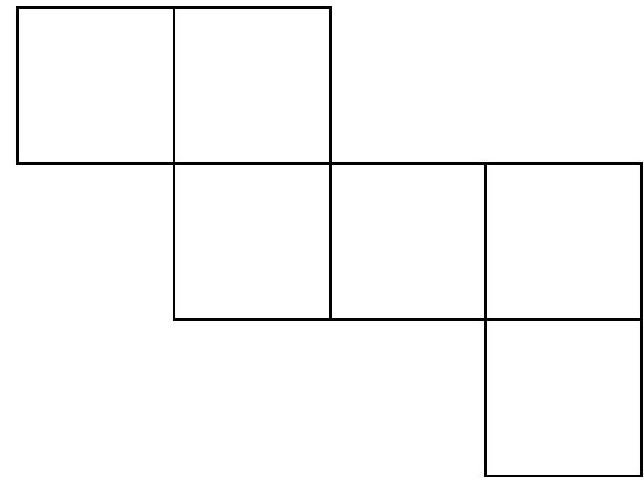
\includegraphics[max width=\textwidth, center]{2024_11_21_1d3b8ece52cfa609efbfg-1(1)}

\section*{Zadanie 3.}
Dany jest taki trójkąt równoramienny, w którym miara każdego kạta wyraża się naturalną liczbą stopni. Miara kąta pomiędzy ramionami tego trójkąta wyraża się pewną liczbą stopni.\\
Uzasadnij, że jest to liczba parzysta.

\section*{Zadanie 4.}
Czworokąty \(A B C D, A B E F, E F D C\) są rombami. Pole trójkąta \(A D F\) jest równe 2.\\
Oblicz pole trójkąta \(B C E\).\\
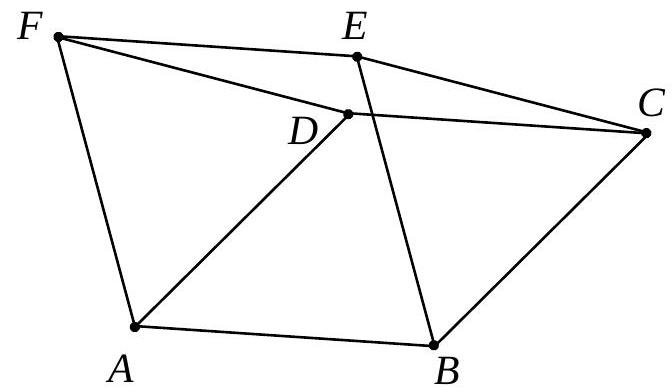
\includegraphics[max width=\textwidth, center]{2024_11_21_1d3b8ece52cfa609efbfg-1}

\section*{Zadanie 5.}
Niektóre liczby w dodawaniu ułamków zwykłych zasłonięto kartami. Wszystkie zasłonięte liczby są naturalne i dodatnie. Jaką liczbę zasłonięto szarą kartą? Ile rozwiązań ma to zadanie?

\[
\frac{\square}{3}+\frac{\square}{5}+\frac{\square}{\square}=\frac{1}{\square}
\]


\end{document}